\documentclass[sigconf]{acmart}

\usepackage{booktabs}
\usepackage{siunitx}
\usepackage{graphicx}
\usepackage{amsmath}

\newcommand{\MatcherLadderCorpusFixes}{42,654}
\newcommand{\MatcherLadderPseudoExamples}{29,411}
\newcommand{\MatcherLadderRows}{%
M1 & Connected baseline & 90.44\% & 32.35\% & 131.8 & 9.225 \\%
M2 & Nearest + street-ref continuity & 93.96\% & 23.22\% & 80.7 & 9.511 \\%
M3 & M2 + connected-candidate gate & 90.76\% & 23.40\% & 131.8 & 9.856 \\%
M4 & Corridor raw mini-HMM & 85.59\% & 17.02\% & 131.8 & 9.521 \\%
M5 & Corridor-aware final & 90.15\% & 53.63\% & 131.8 & 9.093 \\%
M6 & M2 + urban consecutive distance-gap release & 93.96\% & 23.34\% & 80.7 & 8.725 \\%
M7 & M6 + 10m search window & 94.28\% & 25.09\% & 80.7 & 8.488 \\%
M8 & M6 + no-ref street-name continuity & 93.92\% & 23.59\% & 80.7 & 9.429 \\%
M9 & M8 + guarded stale-ref suppression & 93.97\% & 23.59\% & 80.7 & 9.399 \\%
M10 & M9 + node-direction-aware junction release & 93.98\% & 23.65\% & 80.7 & 10.046 \\%
M11 & M10 + topology-free particle sequence & 93.45\% & 25.47\% & 131.8 & 10.087 \\%
M12 & M11 + 10-fix Viterbi sequence & 94.24\% & 26.91\% & 170.9 & 10.374 \\%
Valhalla & Valhalla oracle & 94.04\% & 26.03\% & 155.4 & 7.843 \\
}


\setcopyright{acmlicensed}
\acmConference[SIGSPATIAL '26]{The 34th ACM SIGSPATIAL International Conference on Advances in Geographic Information Systems}{November 3--6, 2026}{Riverside, CA, USA}
\acmYear{2026}
\acmISBN{979-8-4007-XXXX-X/2026/11}
\acmDOI{10.1145/XXXXXXX.XXXXXXX}
\acmBooktitle{Proceedings of the 34th ACM SIGSPATIAL International Conference on Advances in Geographic Information Systems (SIGSPATIAL '26), November 3--6, 2026, Riverside, CA, USA}

\title{Offline Speed-Limit Inference on Smartphones: A Geospatial Systems Benchmark and Deployment Experience [Experiment]}

\author{Raphael Volz}
\affiliation{%
  \institution{Pforzheim University}
  \city{Pforzheim}
  \country{Germany}}
\email{raphael.volz@hs-pforzheim.de}

\begin{document}

\begin{abstract}
Smartphone speed-limit assistance is a geospatial systems problem as much as a map-matching problem. A useful mobile runtime must package country-scale OpenStreetMap data, preserve enough road and locality context for legal speed inference, update efficiently under daily map churn, and still resolve road candidates within the latency and storage envelope of consumer devices. This paper reports a deployment-oriented benchmark and experience study of YouSpeed, an offline-first smartphone runtime for speed-limit inference from OpenStreetMap. We evaluate four runtime data architectures for country-scale lookup, then separate that data-layer result from a route-level replay study of lightweight matcher profiles on current driving logs. The data-layer benchmark shows that a single-file SQLite/RTree artifact is the most stable current representation: on a physical iPhone at the benchmark probe, it answers hybrid road queries in \SI{24.10}{ms} and residential area-context lookup in \SI{0.74}{ms}, and on a stratified Baden-Wuerttemberg iPhone-simulator rerun it answers median hybrid queries in \SI{4.37}{ms}. The Android emulator rerun exposes a portability constraint: the target SQLite distribution must provide RTree support or fall back to non-RTree paths. The route-level replay benchmark covers 21 logs, 42,654 fixes, and 29,411 hindsight labels. It shows that the strongest current lightweight profile reaches 94.28\% replay accuracy and 25.09\% changed-example recall on an 80.7 MiB bundle with \SI{8.488}{ms} query p95, while a heavier 10-fix sequence profile recovers more changed examples but requires a 170.9 MiB bundle. A Valhalla-based oracle reaches 94.04\% replay accuracy and 26.03\% changed-example recall on a 155.4 MiB tile set, making it a useful ceiling check but not a clear replacement for the purpose-built artifact contract. The main lesson is that deployment tradeoffs for mobile geospatial inference should be measured jointly across spatial packaging, update locality, route replay quality, and artifact size; richer graph side tables and route engines do not automatically dominate a well-targeted lightweight spatial runtime.
\end{abstract}

\keywords{mobile GIS, OpenStreetMap, spatial indexing, map matching, intelligent speed assistance, edge spatial computing}

\ccsdesc[500]{Information systems~Geographic information systems}
\ccsdesc[500]{Information systems~Mobile information processing systems}
\ccsdesc[300]{Applied computing~Transportation}

\maketitle

\section{Introduction}

OpenStreetMap (OSM) makes global road-network data available for mobile applications, but using it for driver-facing speed-limit inference is not a simple nearest-road lookup. Speed evidence is distributed across explicit \texttt{maxspeed} tags, inherited regulatory tags, road classes, tunnel and service-road tags, and locality context such as residential polygons or administrative labels \cite{osmwiki_highways,osmwiki_maxspeed}. A smartphone runtime must turn that collaborative, heterogeneous data model into a compact artifact that can be queried offline under intermittent connectivity and mobile storage constraints.

This paper studies that deployment problem through YouSpeed, an offline-first smartphone runtime for OSM-derived speed-limit inference. The runtime is motivated by intelligent speed assistance (ISA), but the contribution here is deliberately narrower than a safety-effect claim. We ask which spatial data representations and lightweight route-matching profiles support low-latency, updateable, auditable speed-limit inference on consumer phones.

An earlier architecture-only formulation treated runtime data representation as the primary result. That framing was useful but incomplete: a single fixed-probe lookup benchmark cannot establish end-to-end speed-limit correctness, and ``S3 is best'' is not surprising without a broader geospatial systems story. This version therefore changes the center of gravity. The architecture benchmark remains the data-layer evidence, but it is now paired with route-level replay, matcher-profile comparison, artifact-size accounting, update analysis, and a Valhalla oracle comparison.

The paper makes three contributions.

\begin{enumerate}
\item We compare four OSM runtime data architectures for offline smartphone speed-limit lookup while holding source data and query modes fixed.
\item We report a route-level replay benchmark over 21 current driving logs, comparing 12 deployable lightweight matcher profiles and a Valhalla oracle under one hindsight-label protocol.
\item We derive deployment lessons for mobile geospatial inference: the best current tradeoff is not the richest graph-bearing matcher, but a lightweight SQLite/RTree bundle with narrow sequence refinements, explicit update contracts, and route replay as the acceptance test.
\end{enumerate}

\section{Related Work}

Map matching has long been studied through geometric, topological, and probabilistic formulations. Surveys and canonical HMM work show why sequence context matters for noisy trajectories \cite{quddus2007,newson2009,lou2009,goh2012,he2013,hunter2014}. Faster variants and precomputed transition schemes such as FMM reduce the route-distance cost of probabilistic matching \cite{yang2018fmm}. Production engines such as OSRM, Valhalla Meili, and Mapbox expose map-matching APIs with candidate radii, transition reasoning, and confidence-style outputs \cite{osrm_match_service,valhalla_meili,mapbox_map_matching_api}.

This paper does not propose a new global map-matching algorithm. Instead, it asks how much sequence and topology machinery is worth carrying inside a smartphone-local speed-limit runtime whose primary data contract is way-keyed inference and updateable OSM-derived bundles. That places the work closer to geospatial systems and mobile spatial data management than to leaderboard-style route reconstruction.

Spatial packaging is also a central related systems topic. R-trees remain the standard indexing mechanism for spatial-window retrieval \cite{guttman1984}; archive-style tile formats such as MBTiles and PMTiles show that physical packaging and distribution are themselves part of applied geospatial system design \cite{mbtiles_spec,pmtiles_docs}. The distinctive issue here is that speed-limit inference couples packaging with legal and locality context: explicit road-speed tags are only one part of the runtime data needed for a phone to infer a speed limit.

OSM-derived mobile systems also inherit an update problem. Daily diffs are small relative to full regional extracts, but they are not naturally aligned with application-specific spatial indexes, inferred defaults, or precomputed graph side tables. A changed way may touch geometry rows, area-context lookup, tile membership, and route-transition support. For a mobile application, the relevant question is therefore not only whether a diff can be parsed, but whether the deployed artifact can be refreshed atomically, validated cheaply, and recovered after partial failure. This paper treats update locality as part of the benchmark because a fast offline index that requires frequent full-bundle replacement is an unattractive mobile contract.

\section{System Overview}

The implemented runtime has three layers. First, an off-device pipeline ingests OSM extracts, keeps car-drivable ways, normalizes speed-related tags, builds residential area-context tables, and emits regional SQLite bundles. Second, mobile clients discover and activate bundles through manifests, country catalogs, checksums, and coverage metadata. Third, the live runtime resolves each GPS fix to a candidate way and derives the speed limit from the selected way, locality context, country code, and bundled penalty rules.

\begin{figure}[t]
\centering

\includegraphics[width=\linewidth]{../../youspeed.de-paper/share/TECHNICAL_ARCHITECTURE_PAPER_SCOPE.png}
\caption{Paper-scope architecture. The evaluated path is OSM-derived bundle publication, mobile bundle activation, local lookup, and replay analysis. The broader observation-sync stack is outside this paper's evidence.}
\Description{A layered architecture diagram showing OSM preprocessing, bundle publication, mobile local lookup, and observation or replay paths.}
\label{fig:architecture}
\end{figure}

Table~\ref{tab:runtime_mapping} summarizes the key normalization step. The mobile runtime does not consume raw OSM nodes, ways, and relations directly. It consumes a query-oriented view: way rows, geometry rows, RTree bounding boxes, area-context polygons, optional graph side tables, optional corridor tables, and manifest metadata.

\begin{table}[t]
\caption{OSM-to-runtime normalization used by the mobile system.}
\label{tab:runtime_mapping}
\centering
\scriptsize
\begin{tabular}{p{2.05cm}p{2.55cm}p{3.0cm}}
\toprule
OSM-side structure & Runtime representation & On-device role \\
\midrule
Car-drivable ways with speed, class, ref, tunnel, and service tags & \texttt{ways}, \texttt{way\_geom}, \texttt{ways\_rtree} & Candidate retrieval, geometry scoring, speed derivation. \\
Residential and place polygons & \texttt{areas}, \texttt{areas\_rtree} & Built-up context and city labels. \\
Shared endpoints and repeated refs & \texttt{way\_links} & Optional connected-transition gating. \\
Tunnel and motorway chains & \texttt{corridor\_progress}, \texttt{corridor\_pairs} & Optional portal-aware sequence reasoning. \\
Coverage and release metadata & Bundle manifests and country catalogs & Bundle routing, checksums, updates, rule selection. \\
\bottomrule
\end{tabular}
\end{table}

The current Germany artifact illustrates why locality fallback is operationally important. In the evaluated snapshot, Germany contains 7,963,481 car-drivable ways, but only 2,639,693 carry explicit speed-limit tags. After rule-aware fusion, explicit tagged limits cover 33.15\% of ways, inherited regulatory tags add 0.98\%, and 65.87\% require context-based fallback. Across 45 European extracts, the median explicit \texttt{maxspeed=*} share is only 16.15\%, with a range from 3.10\% to 67.75\%. An offline runtime therefore needs both road lookup and area-context lookup; explicit speed-tag retrieval alone is insufficient.

\subsection{Artifact Contract}

The mobile artifact contract is intentionally narrower than a general routing engine contract. The phone needs local evidence for the currently observed road segment, not turn-by-turn route reconstruction. Each activated bundle must provide: (i) a bounded spatial candidate query around a GPS fix, (ii) enough geometry to disambiguate nearby carriageways and parallel streets, (iii) speed-tag and default-rule inputs, (iv) built-up locality context, and (v) metadata for coverage, versioning, checksums, and rollback. Optional graph tables may improve selected cases, but they also increase bundle size and update surface. The benchmark therefore evaluates graph-bearing additions only when they improve route-level replay enough to justify this larger contract.

This framing also explains why the system keeps update mechanics visible. The runtime cannot assume continuous connectivity, cannot block driving on large downloads, and must tolerate interrupted activation. The database-centered variants support atomic replacement or patch application using a single file and manifest, whereas many-file tile variants need more file-system bookkeeping and more opportunities for inconsistent partial state. These practical details are not separate engineering concerns; they shape which spatial representation is deployable on phones.

\section{Evaluation Design}

The evaluation has two layers because spatial lookup and route-level arbitration answer different questions.

\subsection{Runtime Data Architectures}

The S1--S4 benchmark isolates data packaging and spatial access. All variants are built from the same Germany snapshot and queried through the same modes.

\begin{table}[t]
\caption{Runtime data architectures evaluated in the lookup benchmark.}
\label{tab:architectures}
\centering
\scriptsize
\begin{tabular}{p{0.65cm}p{2.25cm}p{4.65cm}}
\toprule
ID & Artifact & Rationale \\
\midrule
S1 & Global index files & Simple baseline with broad country-scale scans and high I/O pressure. \\
S2 & Content-addressed spatial tile packs & Explicit partitioning for localized reads and tile-level refresh. \\
S3 & Single SQLite/RTree database & One embedded spatial artifact with direct window retrieval. \\
S4 & SQLite/RTree plus tile prefilter & Adds a membership prefilter to prune dense urban candidate sets. \\
\bottomrule
\end{tabular}
\end{table}

The benchmark uses three way-query modes: bounding-box distance, full polyline distance, and a hybrid that pre-ranks by bounding box before refining a top-\(N\) subset by polyline. It also measures \texttt{polycontainment}, a residential-polygon lookup used for built-up context. The earlier architecture measurements use one Berlin probe \((52.5200,13.4050)\), heading \(90^\circ\), \(k=5\), on a MacBook Pro host and a physical iPhone 14 Pro. This fixed-probe design is retained as a control point, but the SIGSPATIAL artifact now adds a stratified probe manifest over dense urban, same-name, same-reference, tunnel, motorway, low-speed, low-GPS, no-match, and distance-fallback cases drawn from replay logs. We rerun that manifest on final Baden-Wuerttemberg S1--S4 artifacts with an iPhone simulator and an Android emulator; Germany-wide S2/S4 artifacts remain pre-submission work.

For reproducibility, the stratified runner stores every raw query-script response and then reports a normalized ``query core'' time:
\[
t_{core}=t_{candidates}+t_{city}+t_{polyline}+t_{rank}.
\]
This excludes script startup and database-open overhead from the host-side subprocess runner while retaining those raw wall-clock values in the output files. The device benchmark remains the authoritative mobile latency result, but the stratified host run is useful for identifying which probe families stress candidate retrieval and polyline refinement.

\subsection{Route-Level Replay and Hindsight Labels}

The matcher evaluation replays logged driving fixes through deployable S3 profiles. For a fix \(t\), the hindsight label protocol looks at the next \(W=5\) logged selections and accepts a pseudo-label only when the future-majority way is stable, appears in the candidate set already visible at \(t\), and has a consecutive future run length of \(L=5\). These labels are not manual ground truth; they are high-confidence a posteriori labels for evaluating ambiguous local candidate choices.

For each profile \(p\), replay accuracy is
\[
a_p = \frac{1}{|R|}\sum_{t \in R}\mathbf{1}\!\left[\hat{y}^{(p)}_t = y_t\right],
\]
where \(R\) is the set of hindsight-labelled replay fixes, \(y_t\) is the hindsight label, and \(\hat{y}^{(p)}_t\) is the profile output. Changed-example recall focuses on cases where the hindsight label differs from the original live selection:
\[
r_p = \frac{1}{|C|}\sum_{t \in C}\mathbf{1}\!\left[\hat{y}^{(p)}_t = y_t\right],
\quad
C = \{t \in R : y_t \ne y^{live}_t\}.
\]

The replay corpus used for the main matcher ladder contains 21 current logs, 42,654 fixes, and 29,411 hindsight labels. It compares 12 in-house profiles and a desktop Valhalla trace-attribute oracle. In-house rows are measured with cached per-fix query time; the Valhalla row uses trace-window p95.

\subsection{Hard-Case Audit Seed}

The hindsight-label protocol is conservative, but it is still automatic. We therefore maintain a separate hard-case seed corpus for manual audit. The seed contains 12 cases sampled from replay and oracle disagreements: tunnel portal and tunnel exit, motorway same-reference ambiguity, same-name and same-reference parallel roads, low-speed intersection fixes, low-GPS fixes, no-match gaps, and distance-fallback cases. Each row records the live selection, any hindsight pseudo-label, any Valhalla oracle output, the coordinates and course, and a reviewer status. The current audit records eight exact-way decisions and four evidence-backed ambiguous cases; these rows are used qualitatively rather than as an aggregate accuracy denominator.

The purpose of the seed corpus is twofold. First, it supplies a small qualitative check on whether automatic metrics are measuring the intended behavior. Second, it localizes future matcher work: if a profile improves changed-example recall by moving tunnel cases but regresses low-speed intersections, that tradeoff should be visible before deployment.

\section{Results}

\subsection{Architecture Benchmark}

Table~\ref{tab:latency} reports the current host/device latency matrix. S3 is the strongest data-layer choice for decision-relevant device queries: \SI{24.10}{ms} for hybrid, \SI{39.16}{ms} for polyline, and \SI{0.74}{ms} for area-context lookup. S2 improves greatly over S1 but carries 109,333 files in the Germany realization. S4's extra prefilter does not pay off on the current workload; on device it is slower than S3 for every decision-relevant mode and regresses especially on bounding-box lookup.

\begin{table}[t]
\caption{Mean latency at the current benchmark coordinate (\si{\milli\second}).}
\label{tab:latency}
\centering
\scriptsize
\begin{tabular}{llrrrr}
\toprule
Run & Mode & S1 & S2 & S3 & S4 \\
\midrule
host & bbox & 5451.24 & 172.21 & 64.74 & 166.26 \\
host & hybrid & 10152.12 & 169.25 & 29.56 & 64.00 \\
host & polyline & 10300.65 & 170.65 & 38.88 & 72.03 \\
host & polycontain & 1.51 & 1.07 & 0.94 & 0.44 \\
\midrule
device & bbox & 4526.75 & 232.58 & 43.77 & 792.13 \\
device & hybrid & 2935.52 & 61.03 & 24.10 & 99.57 \\
device & polyline & 3122.36 & 76.20 & 39.16 & 78.54 \\
device & polycontain & 3.14 & 0.81 & 0.74 & 2.79 \\
\bottomrule
\end{tabular}
\end{table}

The stratified host rerun in Table~\ref{tab:latency_stratified} uses the available Karlsruhe S1 and S3 artifacts and 11 covered probe strata; the Berlin control point is retained in the raw output but excluded from the aggregate because the Karlsruhe artifacts correctly return no candidates there. The result refines the single-probe story. S1 is competitive on bounding-box-only ranking because the file representation can scan enough precomputed metadata cheaply on this small regional artifact. That is not the decision-relevant operating mode, however. Once geometry refinement is enabled, S3 is much more stable: its median p95 core time is \SI{15.14}{ms} for hybrid lookup and \SI{19.15}{ms} for full polyline lookup, compared with \SI{124.46}{ms} and \SI{137.83}{ms} for S1. The worst S3 stratum is the tunnel portal, where 1,660 candidate ways enter the window and full polyline refinement reaches \SI{33.61}{ms}; this is still well below the S1 polyline worst case of \SI{188.27}{ms}.

\begin{table}[t]
\caption{Host-side stratified query-core latency over the available Karlsruhe S1/S3 artifacts. Values summarize 11 covered probe strata; units are milliseconds.}
\label{tab:latency_stratified}
\centering
\scriptsize
% Auto-generated by scripts/run_stratified_latency_benchmark.py
\begin{tabular}{llrrrr}
\toprule
Arch. & Mode & Strata & Median p50 & Median p95 & Worst p95\\
\midrule
S1 & bbox & 11 & 8.330 & 8.490 & 16.130\\
S1 & hybrid & 11 & 123.015 & 124.460 & 135.650\\
S1 & polyline & 11 & 135.855 & 137.830 & 188.270\\
S3 & bbox & 11 & 12.620 & 12.630 & 19.790\\
S3 & hybrid & 11 & 15.005 & 15.140 & 22.230\\
S3 & polyline & 11 & 19.035 & 19.150 & 33.610\\
\bottomrule
\end{tabular}

\end{table}

This table is not a replacement for the device S1--S4 matrix: it is a stress test over realistic hard-case coordinates. Its main value is diagnostic. Bbox-only lookup can understate the cost of an artifact because it does not pay for the geometry operation that distinguishes adjacent carriageways, tunnel portals, and same-name parallel roads. The gap between S1 and S3 on hybrid/polyline modes is therefore more informative than the bbox row.

\begin{figure}[t]
\centering
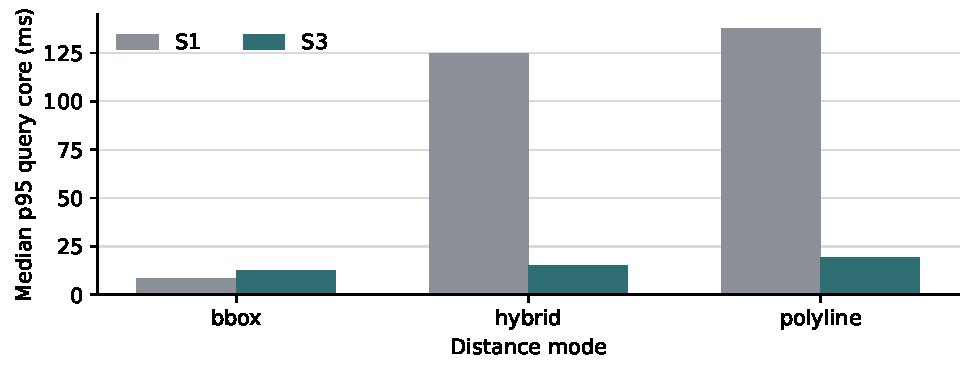
\includegraphics[width=\linewidth]{figures/stratified_latency_p95.pdf}
\caption{Median p95 query-core latency by distance mode on the stratified Karlsruhe S1/S3 host run. Geometry-aware modes expose the file-based S1 cost that bbox-only lookup hides.}
\Description{Grouped bar chart comparing S1 and S3 median p95 query core latency for bbox, hybrid, and polyline modes.}
\label{fig:latency_stratified}
\end{figure}

Table~\ref{tab:device_stratified} reports the corresponding simulator rerun on the final Baden-Wuerttemberg artifact set. On iOS, the RTree-backed S3 path is again the strongest geometry-aware representation: median hybrid latency is \SI{4.37}{ms} and median full-polyline latency is \SI{6.67}{ms} over the 11 covered strata. S4's tile prefilter remains slower than S3 on iOS, suggesting that the extra membership join is not justified for this candidate-window workload. The Android emulator result is useful for a different reason: its platform SQLite build could not load the RTree virtual table in the artifact, so S3 and S4 correctly fell back to S1 and S2 access paths. That is a portability constraint, not a geospatial result, and it should be tested on the target Android SQLite distribution before claiming RTree-backed Android latency.

\begin{table}[t]
\caption{Stratified device latency on final Baden-Wuerttemberg artifacts. Values are median average query times over 11 covered probe strata; units are milliseconds.}
\label{tab:device_stratified}
\centering
\scriptsize
% Derived from ios_sim_stratified_latency_summary.csv and android_emulator_stratified_latency_summary.csv.
\begin{tabular}{llrrrr}
\toprule
Platform & Mode & S1 & S2 & S3 & S4 \\
\midrule
iOS sim. & bbox & 48.29 & 7.09 & 2.38 & 11.56 \\
iOS sim. & hybrid & 48.53 & 8.76 & 4.37 & 12.93 \\
iOS sim. & polyline & 50.37 & 10.40 & 6.67 & 15.67 \\
Android emu. & bbox & 148.96 & 7.19 & 148.34\textsuperscript{a} & 6.98\textsuperscript{a} \\
Android emu. & hybrid & 158.49 & 13.46 & 153.31\textsuperscript{a} & 13.72\textsuperscript{a} \\
Android emu. & polyline & 166.79 & 20.55 & 170.90\textsuperscript{a} & 21.35\textsuperscript{a} \\
\multicolumn{6}{p{7.3cm}}{\textsuperscript{a}Android emulator SQLite reported no usable RTree module for this artifact, so S3 uses the S1 scan fallback and S4 uses the S2 tile fallback.}\\
\bottomrule
\end{tabular}

\end{table}

The update analysis gives the same directional result, but it should be interpreted as a maintenance-cost comparison rather than a universal update-latency benchmark. Over a 30-day Germany daily-diff window, the median day changes more than 61,000 ways and more than 4,600 speed-related tags. The same window invalidates about 2.5 times as many S1 partitions as S2 partitions. For the database-centered variants, exact SQL patch application remains operationally plausible in the current host-side simulation: median V3 patch apply time is about \SI{1.03}{s}, versus about \SI{1.36}{s} for V4.

\begin{table}[t]
\caption{Normalized daily update metrics over the 30-day Germany diff window. S1/S2 replacement bytes use the available Baden-Wuerttemberg artifact references; S3/S4 patch bytes and validation/decompression timings use sampled zlib SQL patch artifacts.}
\label{tab:update_normalized}
\centering
\scriptsize
% Auto-generated by scripts/normalize_update_metrics.py
\begingroup
\setlength{\tabcolsep}{2.4pt}
\begin{tabular}{llrrrrrr}
\toprule
Arch. & Unit & Touch & /1k & Repl. MB & Patch KB & Apply & Val/decomp.\\
\midrule
S1 & partitions & 6728.0 & 109.550 & 915.629 &  &  & \\
S2 & tiles & 2683.5 & 44.297 & 57.239 &  &  & \\
S3 & SQL rows & 131253.0 & 2212.378 &  & 50.182 & 1026.153 & 0.0187/0.5520\\
S4 & SQL rows & 177937.5 & 3005.581 &  & 50.182 & 1358.823 & 0.0187/0.5520\\
\bottomrule
\end{tabular}
\endgroup

\end{table}

The normalized update table deliberately uses different units for partitioned and database-centered artifacts because replacement and patch workflows have different physical contracts. S1 currently implies full reference-artifact replacement of roughly \SI{916}{MB}; S2 can localize that work and has an estimated median tile payload of \SI{57.2}{MB} from the available tile-pack distribution. For S3/S4, sampled SQL patches are much smaller: the median compressed patch is \SI{50.2}{kB}, decompressing to \SI{356.8}{kB}, with median SHA-256 validation and zlib decompression below \SI{1}{ms} on the host. These are not yet full device activation measurements, but they make transferred bytes and integrity/decompression cost visible alongside touched units and apply time.

\begin{figure}[t]
\centering
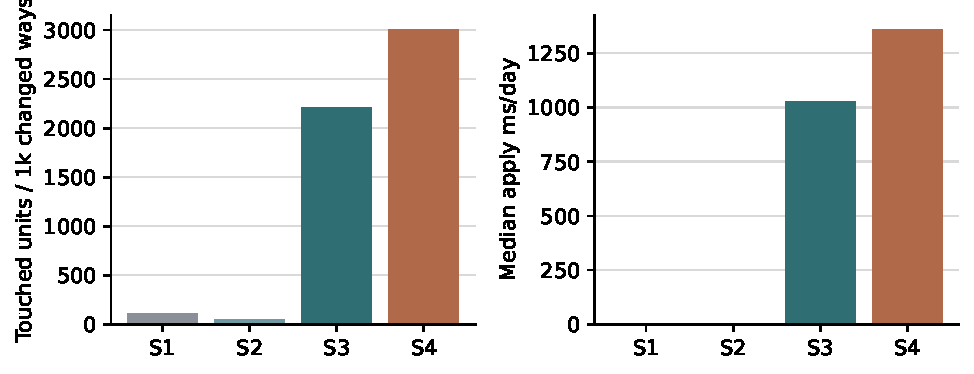
\includegraphics[width=\linewidth]{figures/update_metrics_summary.pdf}
\caption{Normalized update-impact view. Left: touched units per 1,000 changed ways. Right: median host-side patch apply time where measured for S3/S4. Payload and validation/decompression timings are reported in Table~\ref{tab:update_normalized}.}
\Description{Two small bar charts showing normalized touched update units for S1 through S4 and host-side patch apply time for S3 and S4.}
\label{fig:update_metrics}
\end{figure}

\subsection{Causal Matcher Ladder}

The first replay view is a causal complexity ladder over the deployed matcher family. Its purpose is diagnostic: it asks which added mechanisms help before full profile integration. Table~\ref{tab:causal_ladder} shows that added complexity is not monotone. The distance-only baseline already recovers many changed examples; the current deployed final stage is maximally conservative on this corpus, preserving keep-current cases but suppressing all 640 hindsight-labelled switches.

\begin{table}[t]
\caption{Causal matcher-stage ladder over 13 logs and 9,169 hindsight labels.}
\label{tab:causal_ladder}
\centering
\scriptsize
\begin{tabular}{p{3.25cm}rrrr}
\toprule
Stage & Acc. & Chg. rec. & Keep acc. & Net \(\Delta\) \\
\midrule
Distance only & 93.98\% & 57.50\% & 96.72\% & -- \\
Distance + heading & 92.44\% & 43.59\% & 96.11\% & -141 \\
Continuity trace & 90.96\% & 48.91\% & 94.11\% & -136 \\
Corridor/tunnel selectable & 90.99\% & 48.91\% & 94.15\% & +3 \\
Runtime heuristic & 92.67\% & 1.09\% & 99.54\% & +154 \\
Raw mini-HMM pick & 93.57\% & 38.44\% & 97.70\% & +82 \\
Current deployed final & 93.02\% & 0.00\% & 100.00\% & -50 \\
\bottomrule
\end{tabular}
\end{table}

This result matters because it prevents a simple ``more state is better'' conclusion. The current runtime's late hold logic is useful for stability, but not the best hindsight selector. Full profile replay is therefore needed before making a deployment choice.

\subsection{Deployable Runtime Profiles}

Table~\ref{tab:profile_comparison} reports the deployment-facing ladder. The best lightweight row is M7: it reaches 94.28\% replay accuracy and 25.09\% changed-example recall on the same 80.7 MiB no-\texttt{way\_links} bundle tier as M2, while lowering p95 from \SI{9.511}{ms} to \SI{8.488}{ms}. M12 recovers more changed examples at 26.91\%, but requires a 170.9 MiB full bundle and raises query p95 to \SI{10.374}{ms}. M3 shows that simply reintroducing the connected-candidate gate is not worthwhile; it increases artifact tier while underperforming M2. Corridor-heavy rows are also unattractive as general profiles: M5 recovers many changed cases but does so at much lower aggregate replay accuracy.

\begin{table*}[t]
\caption{Unified matcher ladder on the 21-log replay corpus (\MatcherLadderCorpusFixes{} fixes; \MatcherLadderPseudoExamples{} hindsight labels).}
\label{tab:profile_comparison}
\centering
\scriptsize
\begin{tabular}{lp{5.1cm}rrrr}
\toprule
Exp. & Profile & Replay acc. & Changed rec. & Bundle (MiB) & Query p95 (ms) \\
\midrule
\MatcherLadderRows
\bottomrule
\end{tabular}
\end{table*}

The Valhalla oracle is a useful systems reference. On the same seed-bundle replay, it reaches 94.04\% replay accuracy and 26.03\% changed-example recall at \SI{7.843}{ms} p95 on a 155.4 MiB tile set. That is competitive, but it does not reveal an obvious 99\% route-level ceiling or dominate the best in-house tradeoff. A later full Baden-Wuerttemberg rerun leaves the accuracy and changed-recall ranking essentially unchanged while expanding the Valhalla tile set to 725 MiB. For this product contract, Valhalla remains a valuable comparator rather than a clear replacement for a way-keyed, updateable mobile artifact.

\subsection{Hard-Case Corpus Status}

Table~\ref{tab:hard_cases} summarizes the seeded manual-audit corpus. The rows are intentionally not reported as an accuracy number: eight now have an audited exact way id, while four are marked ambiguous with an evidence note because the available fix quality or local geometry does not support a defensible single-way decision. For each row, the repository records live, pseudo-label, Valhalla, and S3 top-candidate outputs. Several examples illustrate why this matters. In the tunnel portal cases, S3's top candidate follows a nearby surface street while the live and pseudo-label rows remain on the tunnel way; this is exactly the sort of case where a portal-aware sequence rule may be justified. In same-reference cases, the automatic sources can disagree even when all labels share a street or route ref, so simple ref agreement is not sufficient ground truth. In low-GPS and stationary cases, the audit deliberately records ambiguity rather than a forced way id.

\begin{table}[t]
\caption{Seeded hard-case families after manual audit. Audited rows have an evidence-backed exact way id; ambiguous rows have an evidence note but no forced way id.}
\label{tab:hard_cases}
\centering
\scriptsize
% Auto-generated by scripts/build_hard_case_context.py
\begin{tabular}{p{4.7cm}rrr}
\toprule
Hard-case family & Seeded & Audited & Ambig.\\
\midrule
Distance fallback / unnamed road & 1 & 0 & 1\\
Low GPS, high uncertainty & 1 & 0 & 1\\
Low-speed intersection & 1 & 0 & 1\\
Motorway same-reference & 1 & 1 & 0\\
No-match gap & 1 & 1 & 0\\
Same-name release & 1 & 1 & 0\\
Same-reference parallel & 1 & 1 & 0\\
Tunnel low-speed exit & 1 & 1 & 0\\
Tunnel portal & 1 & 1 & 0\\
Urban dense, low GPS & 1 & 0 & 1\\
Urban same-name parallel & 1 & 1 & 0\\
Urban unnamed-to-named transition & 1 & 1 & 0\\
\bottomrule
\end{tabular}

\end{table}

This corpus is small by design. A dozen reviewed examples will not replace replay metrics, but it can catch failure modes that a single aggregate score hides. It also gives reviewers a concrete path from observed route-level errors to specific mechanisms: tunnel entry gates, same-ref bounce control, low-speed hold logic, and no-match recovery.

\begin{figure}[t]
\centering
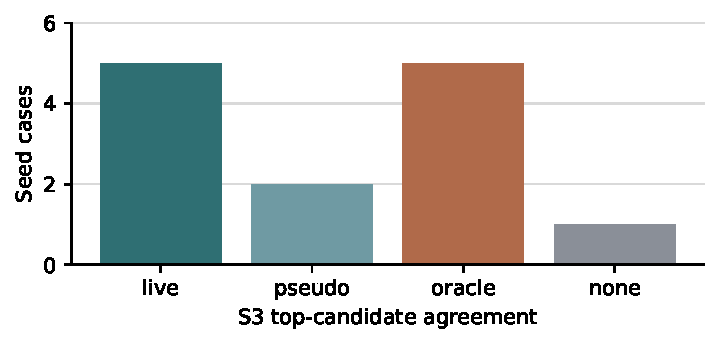
\includegraphics[width=0.82\linewidth]{figures/hardcase_top_candidate_agreement.pdf}
\caption{Agreement between the S3 top candidate and automatic reference sources over the 12 seeded hard cases. Multiple reference sources can match one case; nonmatches identify cases that need manual inspection rather than automatic scoring.}
\Description{Bar chart counting seeded hard cases where the S3 top candidate matches the live label, hindsight pseudo-label, Valhalla oracle, or none of those sources.}
\label{fig:hardcase_agreement}
\end{figure}

\subsection{Qualitative Hard-Case Examples}

The seeded cases also clarify which errors matter for speed-limit inference and which are merely way-id disagreements. In the Gernsbach tunnel cases, the live runtime and hindsight label stay on \texttt{Tunnel Gernsbach (B 462)}, while the S3 top candidate and Valhalla oracle select nearby \texttt{Gottlieb-Klumpp-Strasse} surface segments for several fixes. This is a high-value audit target because the two alternatives plausibly imply different legal context, different built-up inference, and a different expectation for signal loss near the portal. A geometry-only nearest candidate is not enough; the sequence model needs to know whether the trajectory is entering, inside, or leaving a tunnel corridor.

The same-reference cases show a different failure mode. In the \texttt{Tiefenbronner Strasse (K 9800)} example, S3's top candidate agrees with the live way, while both the hindsight pseudo-label and Valhalla oracle point to another way on the same named/reference road. This may or may not matter for the final speed limit: if both OSM ways carry the same speed evidence, a way-id mismatch is less harmful than a speed-rule mismatch. The audit protocol therefore records the correct way id but should also record whether the inferred speed limit would change. That distinction is important for reviewers because the application goal is speed-limit inference, not route reconstruction for its own sake.

The low-speed and low-GPS examples are the cases where a forced label is most dangerous. At the Pforzheim low-speed start, the S3 top candidate and Valhalla oracle both select August-Kayser-Strasse, but the live way id is different and the vehicle is stationary. At a separate low-GPS case on Westtangente (B~463), the horizontal accuracy is nearly \SI{90}{m}. The audit marks these rows ambiguous unless a wider trace window makes the road unambiguous. Treating them as binary errors would reward overconfident matchers.

Finally, motorway same-reference cases highlight the difference between local way selection and deployed user impact. In the A~5 example, the live output, hindsight label, and S3 top candidate all choose one A~5 way while Valhalla selects another A~5 way. If both alternatives carry the same speed interpretation, the case is less severe than the tunnel example even though it is a way-id disagreement. This is why the hard-case audit records exact-way evidence now and leaves speed-limit-equivalence annotation as a next review field.

\section{Discussion}

The main systems lesson is that spatial packaging and matcher design are coupled. A route engine with richer graph machinery may be attractive in isolation, but the mobile deployment choice must also account for bundle size, update artifacts, local overrides, coverage routing, and cross-platform parity. Conversely, a fast spatial lookup benchmark is insufficient unless the resulting artifact supports route-level behavior that can be measured on driving logs. The stratified lookup benchmark reinforces this: a representation can look good under bbox-only retrieval and still be unattractive once the geometry refinement needed for hard cases is included.

The current best tradeoff is therefore narrow but actionable. S3 is the stable data layer on the iOS artifact path: one embedded SQLite/RTree artifact is faster and easier to deploy than many-file tiles or tile-prefiltered SQLite under the current benchmark. The Android emulator run adds an implementation caveat rather than overturning that result: the target SQLite distribution must expose RTree support, or the system needs a fallback artifact. On top of the S3 artifact, the lightweight M7 branch is the strongest present deployment candidate because it improves replay quality over M2 without reintroducing \texttt{way\_links}, corridor tables, or a larger graph bundle. Heavier sequence profiles still identify useful hard cases, especially tunnel and transition examples, but their marginal changed-recall gain does not yet justify their artifact cost.

This also changes how future geospatial mobile inference systems should be evaluated. A single number such as nearest-way accuracy or mean lookup latency hides the real tradeoff. For OSM-derived speed inference, a benchmark should report at least four axes: spatial lookup latency, route-level replay quality, artifact size, and update locality. The YouSpeed results show that those axes can disagree.

\subsection{Why Not Just Use a Route Engine?}

The Valhalla comparison is intentionally strong: it uses a mature route engine and a trace-window oracle rather than a weak nearest-edge baseline. Its result is useful precisely because it is competitive but not decisive. Valhalla recovers slightly more changed examples than M7, yet it requires a different artifact contract, a larger tile set in the regional rerun, and additional integration work to reconcile route-engine edges with way-keyed speed-rule inference and local overrides. For a navigation application already built around Valhalla, that tradeoff may be acceptable. For a phone-local speed-limit assistant, the simpler artifact still has engineering advantages as long as replay quality remains comparable.

This is the central deployment lesson: the best algorithmic component is not automatically the best mobile spatial system. The correct comparison must include the data contract, update path, offline behavior, and failure recovery surface. The current evidence says that the purpose-built SQLite/RTree representation plus lightweight sequence refinements is the strongest baseline to beat.

\section{Limitations and Pre-Submission Work}

The current draft has three important limitations. First, the S1--S4 architecture benchmark in Table~\ref{tab:latency} still reports the fixed Berlin control probe from the earlier architecture study. The repository now contains a stratified probe manifest and a Baden-Wuerttemberg S1--S4 device rerun, but the Germany-wide S2/S4 artifacts were not present locally and must still be rebuilt before the submission can claim a final Germany device matrix.

Second, the route-level labels are hindsight pseudo-labels, not manually verified ground truth. They are useful for stable replay comparison because they only accept future-stable candidates already visible at the current fix. A seeded hard-case corpus now covers tunnel, motorway, same-name, same-reference, low-speed, low-GPS, no-match, and distance-fallback cases, and all 12 seed rows have been reviewed. However, four are intentionally ambiguous and the current audit records exact-way evidence rather than a larger manually labelled accuracy corpus.

Third, update metrics now include reference replacement bytes, sampled SQL patch bytes, SHA-256 validation time, and zlib decompression time, but they are still host-side workflow measurements. A final version should add device-side activation, rollback recovery after interrupted downloads, and exact changed-tile payload accounting for S2.

\section{Conclusion}

This paper reframes offline smartphone speed-limit inference as a geospatial systems benchmark and deployment experience. The stable result is that a single SQLite/RTree artifact is the best current data layer for OSM-derived mobile lookup. The newer route-level result is more important: the strongest current deployment profile is not the richest graph-bearing matcher or a general route engine, but a lightweight sequence refinement that stays on an 80.7 MiB artifact while matching or exceeding heavier alternatives on replay accuracy. The broader lesson for SIGSPATIAL is that mobile spatial inference should be evaluated jointly across packaging, indexing, update mechanics, route replay, and artifact size.

\section*{Acknowledgments}

This draft was prepared from the YouSpeed codebase and internal technical-report material. Generative AI assistance was used to restructure and edit the manuscript draft; the author remains responsible for all claims, data, and citations.

\bibliographystyle{ACM-Reference-Format}
\bibliography{references}

\end{document}
